\documentclass[12pt, a4paper]{article} % свойства докуменат
\usepackage[utf8]{inputenc} % хотим нормальную кодировку
\usepackage[T2A]{fontenc} % тип шрифта, по-моему
\usepackage[russian]{babel} % русские буквы и обозначения
\usepackage{graphicx, xcolor} % графика
\usepackage{subfiles} % царская разбивка на много файлов
\usepackage{amsmath} % различные нужные символы, типа \geqslant
\usepackage{amssymb} % еще немного символов
\usepackage{import} % для включения рисунков
\usepackage{titlesec} % для настройки заголовков и секций вообще
\usepackage{caption} % для подписей к рисункам на 2 строки

% комманда для царского добавления в документ векторной графики
\newcommand{\incfig}[1]{%
    \def\svgwidth{\columnwidth}
    \import{figures/}{#1.pdf}
}
\pdfsuppresswarningpagegroup=1

\newcommand\eqdef{\stackrel{\text{\tiny def}}{=}}

% русские знаки нестрогих неравенств
\renewcommand{\le}{\leqslant}
\renewcommand{\ge}{\geqslant}

\newcommand{\sectionbreak}{\clearpage}

\titleformat{\section}{\normalfont\Large\bfseries}{\thesection.}{1em}{}
\titleformat{\subsection}{\normalfont\Large\bfseries}{\thesubsection.}{1em}{}

\DeclareMathOperator{\mymod}{mod}
\DeclareMathOperator*{\res}{res}

\graphicspath{figures}

\begin{document}

\subfile{titul.tex}

\tableofcontents

\section{Постановка задачи}

Для функции $f(\cdot)$ одной действительной переменной надо найти
ее преобразование Фурье с помощью алгоритма бытрого преобразования Фурье
и сравнить полученное преобразование с вычесленным аналитически.
Исследовать эффекты ряби и наложения спектра, возникающие при использовании
данного алгоритма.
Для этого необходимо реализовать в системе MATLAB функцию \texttt{plotFT},
принимающую на вход следующие аргументы:
\begin{itemize}
    \item \texttt{hFigure}~---~handle фигуры, куда осуществляется вывод
        графиков,
    \item \texttt{fHandle}~---~handle функции, которую надо преобразовать,
    \item \texttt{fFTHandle}~---~необязательный параметр, handle функции,
        задающей аналитически вычесленное преобразование Фурье,
    \item \texttt{step}~---~шаг дискретизации,
    \item \texttt{inpLimVec}~---~окно для входной функции,
    \item \texttt{outLimVec}~---~необязательный параметр, задающей пределы
        осей для вывода результата преобразования Фурье.
\end{itemize} 

Построить преобразование Фурье для слебующего набора функций:

\begin{enumerate}
    \item $\displaystyle f_1(t) = \frac{2t}{5 - 4t + t^2}$,
    \item $\displaystyle f_2(t) = \left( t^2 + t \right)[t \le 1]$,
    \item $\displaystyle f_3(t) = t^3 e^{-2t^2-t}$,
    \item $\displaystyle f_4(t) =
        \frac{e^{-2\lvert t \rvert }}{1 + 4\left\lvert t \right\rvert ^{5}}$.
\end{enumerate} 

Для функций $f_1(t)$ и $f_2(t)$ сравнить численный результат с аналитическим.

\section{Алгоритм решения}

Пусть задана функция $f(\cdot)$ и окно $[a, b]$.
Положим $T \eqdef b - a$.
В данной задаче это равносильно тому, что функция просто определена на $[a,b]$.
Тогда продолжим  $T$-периодически нашу функцию на $\mathbb{R}$:
\[
    f_0(t) = f\bigl( a + (t-a) \mymod T \bigr),\quad t \in \mathbb{R}
.\] 

Образ $f_0(\cdot)$ при приобразовании Фурье~---~это образ исходной функции,
но умноженный на <<забор>> из дельта-функций, идущих с шагом 
$\Delta_\lambda = 2\pi\!/ T$, причем $\Delta_\lambda$~---~это тот шаг,
с которым мы получим отсчеты преобразования Фурье.

Затем мы вычисляем шаг $\Delta$, с которым мы будем брать отсчеты исходной функции.
Он должен быть, во-первых, не меньше заданного, во-вторых, $T$ должно делиться
на  $\Delta$ нацело.

После того, как шаг выбран, вычсляются отсчеты $f_0[n]$ функции 
$f_0(\cdot)$ на отрезке $[-\Delta\!/ 2, T - \Delta\!/2]$, где 
$n = \overline{1,\ldots,N},\ N =T\!/\!\Delta$.

К отсчетам применяется дискретное преобразование Фурье:

\[
    F[k] = \Delta \underbrace{
        \sum\limits_{n=1}^{N} f[n] \exp{\left(
            \frac{-2\pi i (n-1)(k-1)}{N}
        \right)}
    }_{\text{\normalsize команда \texttt{fft}}}
.\] 

Получаются отсчеты образа Фурье на отрезке $[0, 2\pi\!/\!\Delta]$.
Продолжая $(2\pi\!/\!\Delta)$-периодически, получаем отсчеты на всей прямой
и выводим на график на нужном отрезке.

\section{Аналитическое вычисление преобразования Фурье}
\subsection{1-я функция}

$$\displaystyle f(t) = \frac{2t}{5 - 4t + t^2}.$$

Используя теорему о вычетах, вычислим преобразование Фурье,
как это описано здесь~\cite[с.~127]{Leon}.
Рассмотрим 3 случая: $\lambda < 0$, $\lambda > 0$ и $\lambda = 0$:

\begin{enumerate}
\item $\lambda < 0$.
    \begin{multline*}
        F(\lambda) =
        \int\limits_{-\infty}^{\infty}
           \frac{2te^{-it\lambda}}{5 - 4t + t^2}\,dt =
        \int\limits_{-\infty}^{\infty}
           \frac{2te^{it\lvert \lambda \rvert}}{5-4t+t^2}\,dt =\\
           2\pi i \sum\limits_{i\colon \Im t_i > 0} \res\limits_{t=t_i}{\frac{2te^{it\lvert \lambda \rvert}}{5-4t+t^2}}        
    \end{multline*}
    Найдем точки, в которых вычет будет отличен от $0$:
     \[
        5 - 4t + t^2 = 0 \iff t = 2 \pm i
    .\] 
    Из этих точек на интересует только $2 + i$, так как у нее положительная
    мнимая часть.
    \[
        \res\limits_{t=2+i} \frac{2te^{it\lvert \lambda \rvert }}{5-4t+t^2} =
        \frac{2(2+i)e^{i(2+i)\lvert \lambda \rvert}}{2i}
    .\] 
    Тогда
    \[
        F(\lambda) = 2\pi(2+i)e^{i(2+i)\lvert \lambda \rvert}
    .\] 
    И, наконец, учитывая, что $\lambda < 0$, получаем:
\begin{multline*}
        F(\lambda) = 2\pi(2+i)e^{(1-2i)\lambda} =\\
        2\pi e^\lambda\left[ 2\cos(2\lambda) + \sin(2\lambda) +
        i\bigl( \cos(2\lambda) - 2\sin(2\lambda) \bigr)\right]
.\end{multline*}

\item $\lambda > 0$.
    В таком случае сделаем замену $z = -t$.
    Минус вылезет 3 раза: из-под дифференциала, из пределов и из $t$ в знаменателе.
    Получаем:
     \[
        F(\lambda) = -\int\limits_{-\infty}^{\infty} 
            \frac{2ze^{iz\lambda}}{z^2 + 4z + 5}\,dz =
        -2\pi \sum\limits_{i\colon \Im z_i > 0} \res\limits_{z=z_i}
            \frac{2ze^{iz\lambda}}{z^2 + 4z + 5}
    .\] 

    Находим особые точки:
    \[
        z^2 + 4z + 5 = 0 \iff z = -2 \pm i
    .\] 
    Из них нас интересует только точка $-2 + i$:
     \[
        \res\limits_{z = -2+i} \frac{2ze^{iz\lambda}}{z^2 + 4z + 5} =
        \frac{2(-2+i)e^{i(-2+i)\lambda}}{2i}
    .\] 
    Получаем 
    \begin{multline*}
        F(\lambda) = 2\pi (2 - i)e^{-(1+2i)\lambda} =\\
        2\pi e^{-\lambda}\left[ 2\cos(2\lambda) - \sin(2\lambda) 
        -i \bigl( \cos(2\lambda) + 2\sin(2\lambda) \bigr)\right]
    .\end{multline*}
    
\item $\lambda = 0$.

    В этом случае подынтегральное выражение ведет себя как 
    $1\!/ t + \overline{o}(1\!/ t)$ и несобственный интеграл расходится
    даже в смысле главного значения.
    Поэтому в действительной части у образа нашей функции устранимый разрыв,
    а в мнимой~---~разрыв 2 рода.
\end{enumerate} 

\subsection{2-я функция}

$$\displaystyle f(t) = (t^2+t)\bigl[|t| \le 1\bigr].$$

Для начала разобьем интеграл на 2:

\[
    F(\lambda) =
    \int\limits_{-\infty}^{\infty} f(t)e^{-it\lambda}\,dt =
    \int\limits_{-1}^{1} (t^2 + t) e^{-it\lambda}\,dt =
    \int\limits_{-1}^{1} t^2 e^{-it\lambda}\,dt +
    \int\limits_{-1}^{1} t e^{-it\lambda}\,dt
.\] 

Послдений интеграл обозначим за $I$, а первый выразим через него, взяв по частям:

 \[
    \int\limits_{-1}^{1} t^2 e^{-it\lambda}\,dt = 
    \left. -\frac{t^2e^{-it\lambda}}{i\lambda} \right|_{-1}^1 +
        \frac{2}{i\lambda} I =
    \frac{2}{\lambda}\bigl(\sin(\lambda) - iI\bigr)
.\]

Теперь вычислим $I$:

 \[
    I = \left. -\frac{te^{-it\lambda}}{i\lambda} \right|_{-1}^1 +
        \frac{1}{i\lambda} \int\limits_{-1}^{1} e^{-it\lambda}\,dt =
    \frac{2i\cos(\lambda)}{\lambda} - \frac{2i\sin(\lambda)}{\lambda^2}
.\] 

Тогда при $\lambda \neq 0$ имеем:

\begin{equation*}
    F_0(\lambda) = 
    \frac{2}{\lambda^3} \left( \lambda^2\sin(\lambda) + 2\lambda\cos(\lambda)
    - 2\sin(\lambda)\right) +
    \frac{2i}{\lambda^2} \bigl( \lambda\cos(\lambda) - \sin(\lambda)\bigr)
.\end{equation*}

Вычислим интеграл явно при $\lambda = 0$:

 \[
    \int\limits_{-1}^{1} (t^2 + t)\,dt = 
    \left. \left(\frac{t^3}{3} + \frac{t^2}{2}\right) \right|_{-1}^1 =
    \frac{2}{3}
.\]

Окончательно:

\[
    F(\lambda) = 
    \begin{cases}
        F_0(\lambda), &\text{если} \ \lambda \neq 0, \\
    \frac{2}{3}, & \text{иначе}
    \end{cases} 
.\] 

\section{Графики}

В этом разделе сначала демонстрируются графики преобразований Фурье для 
качественного подбора параметров для заданнных функций, а потом исследуются
некоторые искажения и варианты их устранения.

\subsection{Результаты для заданных функций}

Графики преобразования Фурье для заданных функций показаны на рис.~\ref{fig:func1}--\ref{fig:func4}.

\begin{figure}[b]
    \centering
    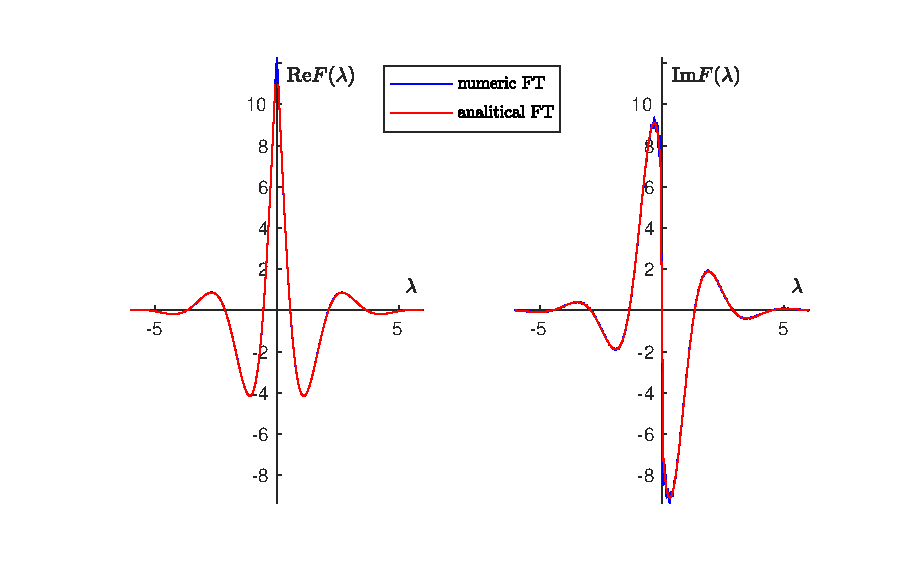
\includegraphics[width=\textwidth]{figures/func1.eps}
    \caption{ПФ для $f_1(t) = \frac{2t}{5 - 4t + t^2}$.\\
    $a = -50,\ b = 50,\ \Delta = 0.01$.}
    \label{fig:func1}
\end{figure}

\begin{figure}[b]
    \centering
    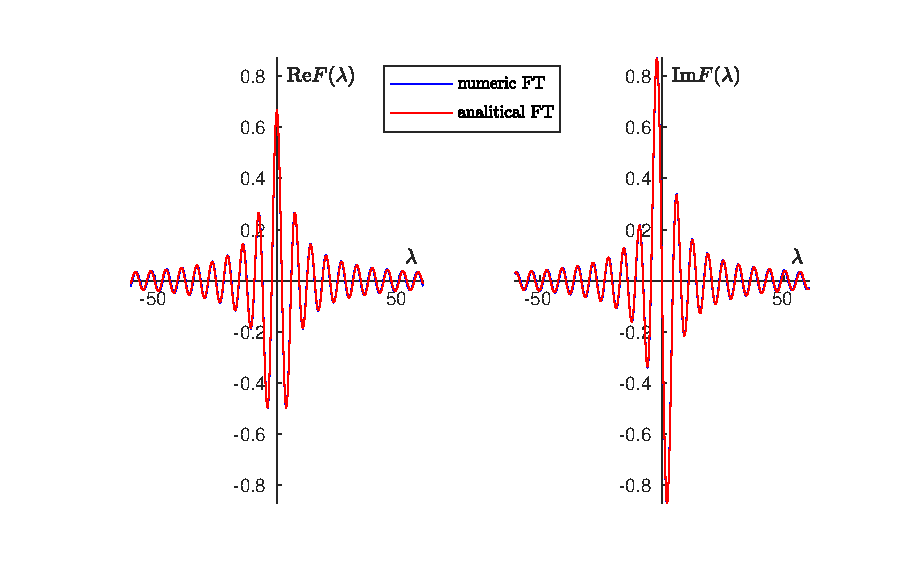
\includegraphics[width=\textwidth]{figures/func2.eps}
    \caption{ПФ для $f_2(t) = \left( t^2 + t \right)[t \le 1]$.\\
    $a = -10,\ b = 10,\ \Delta = 0.01$.}
    \label{fig:func2}
\end{figure}

\begin{figure}[b]
    \centering
    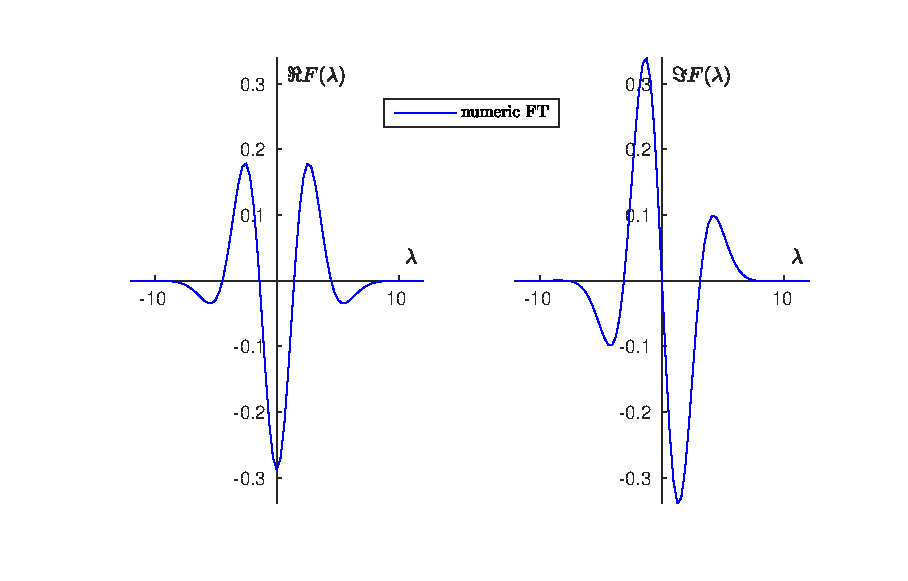
\includegraphics[width=\textwidth]{figures/func3.eps}
    \caption{ПФ для $f_3(t) = t^3 e^{-2t^2-t}$.\\
    $a = -10,\ b = 10,\ \Delta = 0.01$.}
    \label{fig:func3}
\end{figure}

\begin{figure}[b]
    \centering
    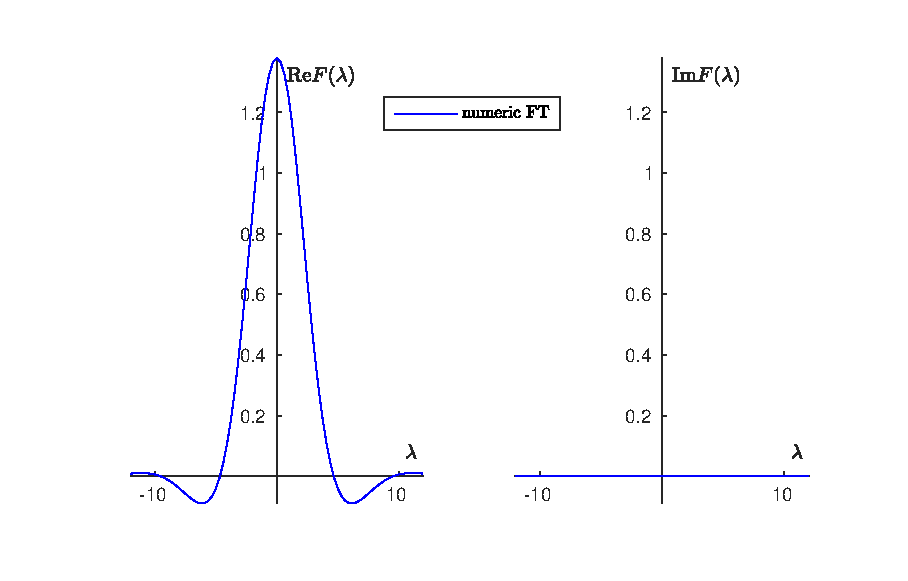
\includegraphics[width=\textwidth]{figures/func4.eps}
    \caption{ПФ для $f_4(t) =
        \frac{e^{-2\lvert t \rvert }}{1 + 4\left\lvert t \right\rvert ^{5}}$.\\
    $a = -10,\ b = 10,\ \Delta = 0.01$.}
    \label{fig:func4}
\end{figure}

\subsection{Эффект ряби}

Эффект ряби возникает из-за невозможности точно посчитать несобственный интеграл.
Теоритически этот эффект возникает при выборе окна исходной функции.
При преобразовании Фурье умножение на окно становится сверткой с чем-то,
похожим на $\frac{\sin(x)}{x}$.
В точках непрерывности можно добиться сколь угодно малой ряби выбором большого окна (см. рис.~\ref{fig:ripple1}, \ref{fig:ripple2}),
а в точках разрыва функции-образа убрать рябь подбором параметров невозможно 
(см. рис.~\ref{fig:func1} и~\ref{fig:ripple3}, рябь вблизи нуля в мнимой части).

\begin{figure}[b]
    \centering
    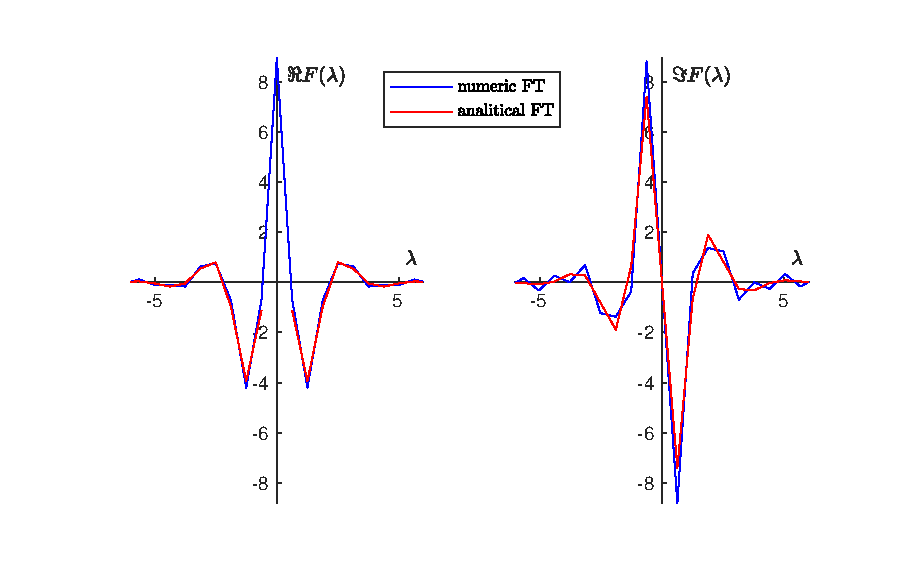
\includegraphics[width=\textwidth]{figures/ripple1.eps}
    \caption{Эффект ряби для $f_1(\cdot)$.\\
    $a = -5,\ b = 5,\ \Delta = 0.1$.}
    \label{fig:ripple1}
\end{figure}

\begin{figure}[b]
    \centering
    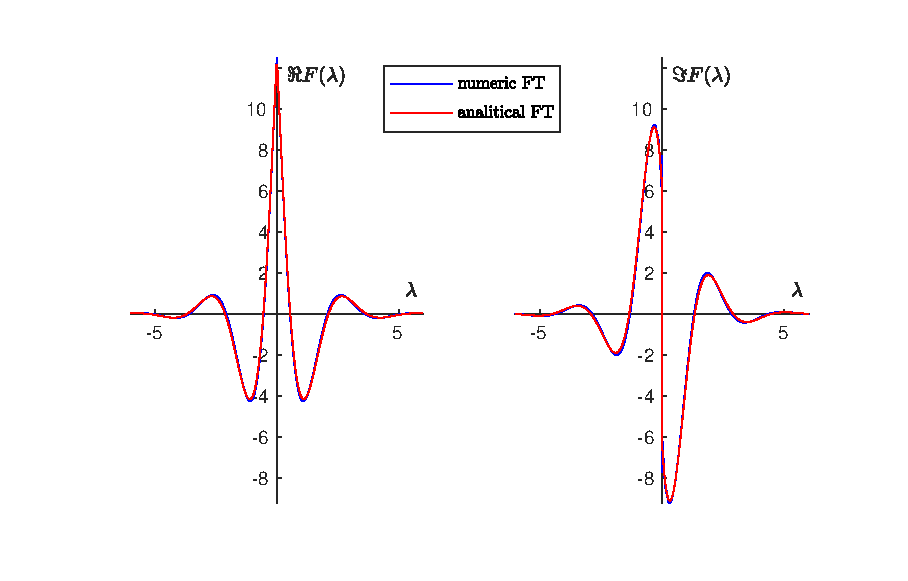
\includegraphics[width=\textwidth]{figures/ripple2.eps}
    \caption{
    Устранение ряби для $f_1(\cdot)$ путем расширения окна.\newline
    $a = -200,\ b = 200,\ \Delta = 0.1$.}
    \label{fig:ripple2}
\end{figure}

\begin{figure}[b]
    \centering
    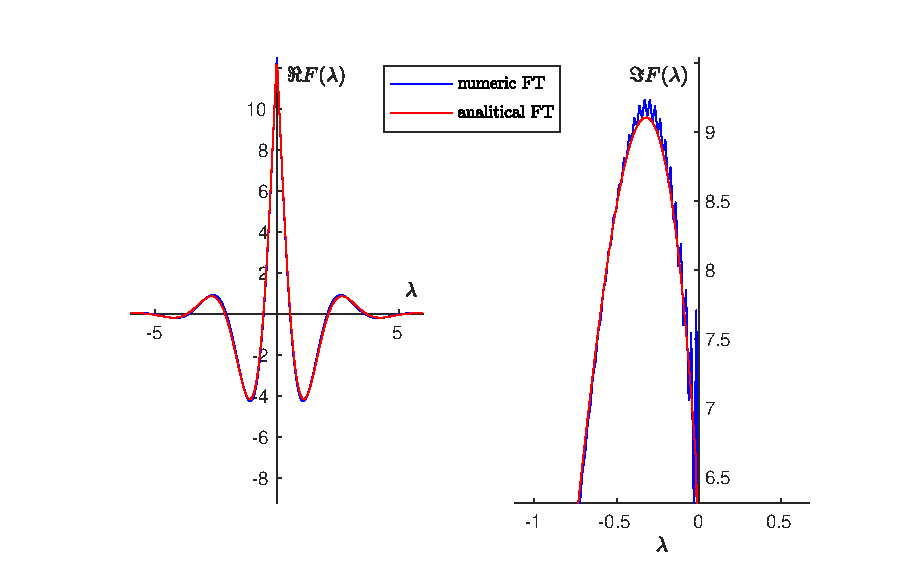
\includegraphics[width=\textwidth]{figures/ripple3.eps}
    \caption{
    Но вблизи точек разрыва образа $f_1(\cdot)$ рябь неустранима.\newline
    $a = -200,\ b = 200,\ \Delta = 0.1$.}
    \label{fig:ripple3}
\end{figure}

\subsection{Эффект наложения спектра}

Эффект наложения спектра возникает в момент, когда мы выбираем шаг сетки для прообраза.
В теории отсчеты функции символизируются умножением на <<забор>> из дельта-функций,
который при преобразовании Фурье переходит в <<забор>>, но с шагом $2\pi\!/\!\Delta$.
Операция умножения становится сверткой и в итоге образом становися исходных
образов, но сдвинутых на некоторое число периодов $2\pi\!/\!\Delta$.
Соответственно, выбирая большой шаг, мы уменьшаем период образа и он
<<не успевает прижаться к нулю>>.
На рис.~\ref{fig:aliasing} в качестве примера рассмотрена только действительная часть образа Фурье для функции $f_1(\cdot)$.

\begin{figure}[b]
    \centering
    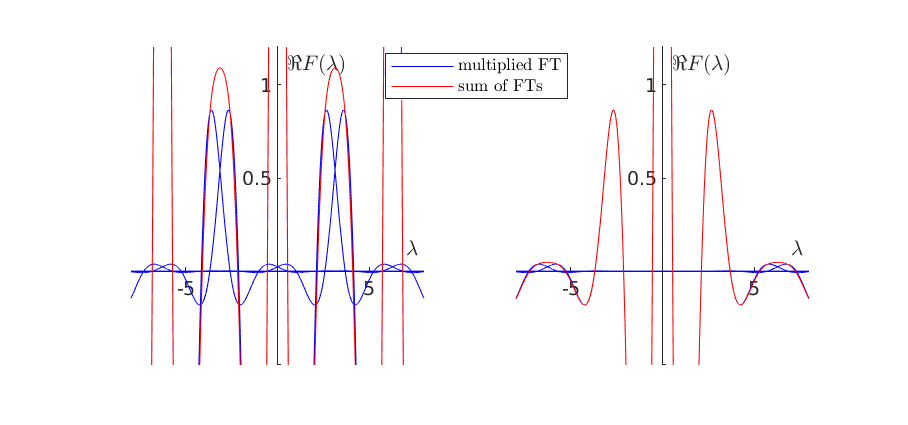
\includegraphics[width=\textwidth]{figures/aliasing.eps}
    \caption{
        На левом графике показаны размноженный образ Фурье и сумма образов при шаге
        $\Delta = 1$, виден ярко выраженный эффект наложения спектра.
        На правом графике выбран шаг $\Delta=1\!/\!2$, и эффект практически отсутствует.
    }
    \label{fig:aliasing}
\end{figure}

\bibliographystyle{utf8gost705u}
\bibliography{biblio}

\end{document}
